% !TEX root = SocialVision2012.tex

\subsection{Multi-source multi-view network estimation}
\label{sec:vis2net}

In addition to analyzing social interactions in videos, we will investigate tools for analyzing social \emph{relationships}, in the form of the social network that embeds the people observed in an image and video collection. As is customary, we consider the social network of $K$ individuals to be an undirected weighted graph $G$, with $K$ nodes and a non-negative weight in $[0,1]$ on each edge between a node-pair. Each edge weight represents the social proximity, or strength of tie, between two people, and they are conveniently collected in a positive symmetric affinity matrix $A$ of size $K\times K$. As described in Sections~\ref{sec:intro} and \ref{sec:background}, our goal is to develop methods for reconstructing social networks that are well-suited for vision by: 1) incorporating a wide variety of noisy sources (diverse social cues automatically extracted from images and videos of varying quality); 2) modeling the multiple-community structure of many common networks ; and 3) being able to tolerate identity errors and high levels of missing data.

It has commonly been observed that social networks include multiple overlapping communities (overlapping clusters). Computationally this means that the social proximity between a pair of nodes is not scalar-valued but depends on the type of roles or memberships (e.g., friends vs. workmates vs. family) by which it is being considered~(e.g.,~\cite{AiroldiBFX08,Kim12}). We refer to these communities/clusters as different \emph{views} in the network and we represent them by defining $G\triangleq\{A^{(v)}\}_{v=1}^{V}$, where $A^{(v)}$ is the affinity matrix summarizing the ties between every pair of members as measured in the $v$th view. For example, if $v\in\{1,2,3\}$ corresponds to friends, family, and workmates,  $A^{(1)}(i,j)=1$, $A^{(2)}(i,j)=0$, and $A^{(3)}(i,j)=1$ indicates that Alice ($i$) and Bob ($j$) are unrelated but are simultaneously close friends and workmates. The three views overlap in general, and the effective tie between each node pair depends on which view is be used to assess their relationship.

In addition to considering multiple views, we must also account for the fact that social information comes from multiple distinct cues extracted from visual data, and that these cues cannot be automatically associated with people's identities with complete certainty. We represent this using $S$ \emph{sources} that produce socially-informative cues $\vy^s, s=1,2,\cdots,S$, with each $\vy^s(i,j)$ a multi-dimensional descriptor computed from a distinct socially-informative visual cue related to people $i$ and $j$. As an example, for a detected, tracked and correctly-identified pair of individuals Alice $(i)$ and Bob $(j)$, a set of sources could include (possibly time-varying): relative positions of the two detections $\vy^1(i,j)$ (or $\vy^1$ for short);  relative head poses $\vy^2$; relative body poses $\vy^3$; distribution over interaction categories $\vy^4$ recovered as in Section~\ref{sec:activity}; and scene category $\vy^5$. Since limitations of identity recognition from faces etc.~ prevent identities from being known with certainty, each source will generally creates multiple outputs. For example, if we cannot distinguish Bob ($j$) from Charlie ($k$), then each sources will produce two outputs satisfying $\vy^s(i,j)=\vy^s(i,k)$. 

We seek an unified learning-based paradigm to obtain the multi-view network representations (affinity matrices $A^{(v)}$) from multiple, heterogeneous, and noisy visual sources. We refer to this architecture as multi-source multi-view network estimation. To address this problem we will consider architectures consisting of $V$ `oracles' $\Psi_{v}$ that we aim to learn, each of which is an estimator $\hat{A}^{(v)}$ of view $v$ from descriptor $\bar{\vy}=[\vy^1,\vy^2, \cdots,\vy^S]$, i.e., $\hat{A}^{(v)}=\Psi_{v}(\bar{\vy})$. Assume that we have $N$ samples of graphs for which we have computed their visual cues $\{\bar{\vy}_{n}\}_{n=1}^{N}$  from related imagery. Meanwhile, there may (or may not) be another small collection of $M$ sample graphs for which we have computed their visual cues $\{\bar{\vy}_{m}\}_{m=1}^{M}$ and had their `ground-truth' affinities $\{\bar{A}^{(v)}_{m}\}_{m=1}^{M}$ (These ground-truths are available, for instance, through our prototype system as to be introduced in Section \ref{sec:sys}). Then, the overall learning objective can be represented as 
\begin{equation}\label{eq:sensing}
\{\Psi^{*}_{v}\}=\arg\min_{\{\Psi_{v}\},\{\hat{A}^{(v)}_l\}_{l=1}^{N+M}}\sum_{m=1}^{M}\mathcal{J}(\{\Psi_{v}\}, \{\bar{\vy}_m\}, \{\bar{A}^{(v)}_m\})+\tau(\{\hat{A}^{(v)}_m\},\{\hat{A}^{(v)}_n\})+\gamma(\{\Psi_{v}\}).
 \end{equation}
 
Specifically, we use the first term $\mathcal{J}$ to enforce the estimation quality of the oracles on supervised samples, for example, by defining $\mathcal{J}(\{\Psi_{v}\}, \{\bar{\vy}_m\}, \{\bar{A}^{(v)}_m\})=\sum_{v=1}^{V}\|\Psi_{v}(\vy_m)-A^{(v)}_m\|^{2}$,  such that the estimated network is as close as possible to the `ground-truth' in the least square sense. Powerful regression machines exist for the oracles, such as Gaussian process regression \cite{GPbook} or deep learning \cite{DLbook}. However, socially-compatible estimations requires more than conventional estimations, in the sense that the individual oracles must give compatible estimates across views. Two nodes inferred as family members by one oracle, for example, should receive low confidence score from the friendship oracle which claims that they are adversary to each other. We use the penalty $\gamma$ to enforce the compatibility among oracles. Finally, we have been fully aware of the community clustering effects of real-world social networks, and therefore we incorporate penalty $\tau$ to regularize all estimated matrices, and in particular, to enforce the clustering effect within each estimated affinity matrix, so that if node $i$ and node $j$ are both inferred as family members of node $k$ we will have the same inference for the relationship between $i$ and $j$. We will explore optimal formats for $\gamma$ and $\tau$ by, e.g., employing or extending the commonly used network priors summarized in \cite{Goldenberg}. Cross-view compatibility and within-view clustering are essential to the multi-view sensing architecture, which is dissimilar to any other regression machines which accept and output independent samples, and are at the heart of our proposed socially-aware visual sensing paradigm.


%\begin{figure}[t!]
%\begin{center}
%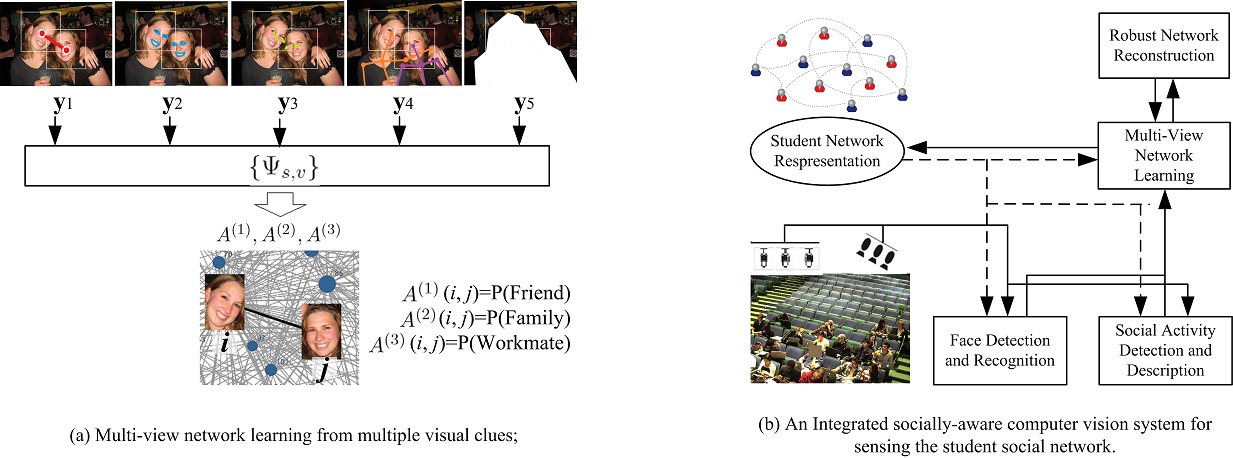
\includegraphics[width=\columnwidth]{featurelearn}
%\end{center}
%\vspace{-0.25in} \caption{\captionsize 
%Illustrations for the problem of multi-view network learning from multiple low-level visual clues and the framework of integrated socially-aware computer vision for understanding student netwrok. \label{fig:featurelearn}\afterfigspace}
%\end{figure}




%%%%%%%%%%%%%%%%%%%%%%%%%%%%%%%%%%%%%%%%%%%%%%%%%%%%%%%%%

\subsubsection{Associating identities with image targets}
\label{sec:assoc}

To obtain the low-level visual descriptions $\vy^s$ between individual $i$ and individual $j$, we must first identify the two individuals from the detections in images or tracks in videos. While the state-of-art face recognizer has achieved compellingly outstanding performance even for the faces `in the wild', there always remain ambiguities and errors. Suppose that from an image we have detected $L$ faces or from a video we have tracked $L$ faces, and that the face recognizer outputs a $K$-dimensional probabilistic histogram $h_l$ for the $l$th target in the image or video, with $h_l(k)$ describing the likelihood for this target to belong to the $k$th identity. We must assign each of these $L$ targets to the possible $K$ identities of interest. 

The problem of uncertainties in node identities is uncommon for conventional social network research, where the nodes are mostly straightforwardly identifiable. However, the problem is unique and crucial for network sensing from image data, because of the nodes in the network are indirectly related to image targets via a face/human detector and/or tracker, especially when we aim to accumulate social evidences from many image/video samples.

We propose to explore robust algorithms that may properly handle the non-robustness of a face recognizer and provide identity assignments that are less sensitive to the erroneous output from a face recognizer. A preliminary solution can be straightforward as follows. Instead of assigning each target to a single identity from $K$ possible ones that might be incorrect, consider that To leverage and properly aggregate these likelihood conveyed from face recognition, we may first enumerate all $\prod_{l=0}^{L-1}(K-l)$ possible assignments. We then may duplicate the original image or video into $\prod_{l=0}^{L-1}(K-l)$ copies, in each of which we may assume that the $L$ targets have a determined identity assignment $\{k_1, k_2, \cdots, k_L\}, k_l\in\{1,2, \cdots, K\}$. We allow all these $\prod_{l=0}^{L-1}(K-l)$ `hallucinated' samples to be used for computing low-level description $\vy^s$, where the $(i,j)$-pair of targets will contribute to the descriptor $\vy^s(k_i,k_j)$, with appropriate pooling strategy to effective and efficiently aggregate all contributions from the expanded set of $\prod_{l=0}^{L-1}(K-l)$ new samples. A `maximum-pooling' approach, for example, may be employed by determining $k_l^{*}=\max_{k}h_l(k)$, the most probable identity for target $l$, and use the only maximum assignment $\{k_1^{*}, k_2^{*}, \cdots, k_L^{*}\}$ to compute the visual cues between individuals specified by $\{k_1^{*}, k_2^{*}, \cdots, k_L^{*}\}$. This strategy is essentially identical to the idea of assigning each target to a single (possibly incorrect) identity. Alternatively, we may adopt a weighted average pooling, where the hallucinated image/video with assignment $\{k_1, k_2, \cdots, k_L\}$ will contribute to the visual cues but with a confidence score, for example, of $\prod_{l=1}^{L}h_l(k_l)$.

We propose to develop and evaluate other systematic solutions during the award period. We foresee that our treatment to this problem may lead to new results in decision theory and statistical signal processing on graphs and other relational data structures.

